\section{IPV6}
\subsection{Adressbildung}
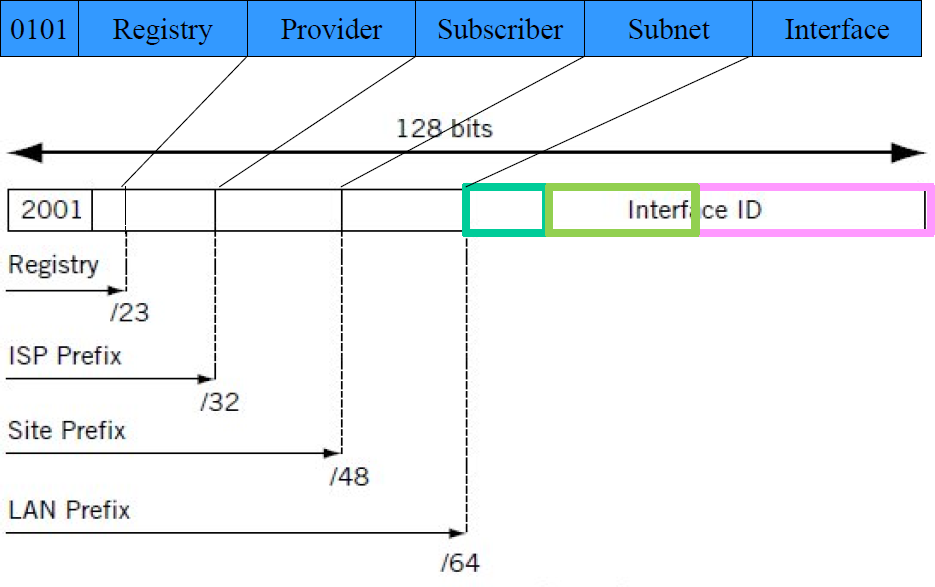
\includegraphics[scale=0.5]{media/ipv6.png}
Präfix + Netzwerkstruktur + Interface-Identifier = 128Bit IPV6 Adresse\\
Prefix + Netzwerkstruktur = 64Bit\\
Interface-Identifier = 3Byte MAC OUI + ff:fe + 3Byte MAC NIC\\
Wobei im MAC OUI Teil das globally administered bit (7bit, $2^{2}$ Position) gesetzt wird.

Beispiel MAC: 58:55:ca:f3:e1:29Y\\
1. ff:fe einfügen: 58:55:ca:ff:fe:f3:e1:29\\
2. Globally administered Bit setzten: 58 = 01010100 => 01010110, 5a\\
3. Resultierende Adresse: 5a55:caff:fef3:e129

\subsubsection*{Vereinfachungen}

- Führende Nullen innerhalb eines Blockes dürfen ausgelassen werden: 2001:0db8:0000:08d3:0000:8a2e:0070:7344 ist gleichbedeutend mit 2001:db8:0:8d3:0:8a2e:70:7344.

- Ein oder mehrere aufeinander folgende Blöcke, deren Wert 0 (bzw. 0000) beträgt, dürfen ausgelassen werden. Dies wird durch zwei aufeinander folgende Doppelpunkte angezeigt: 2001:0db8:0:0:0:0:1428:57ab ist gleichbedeutend mit 2001:db8::1428:57ab.

- Die Reduktion durch Regel 3 darf nur einmal durchgeführt werden, das heißt, es darf höchstens eine zusammenhängende Gruppe aus Null-Blöcken in der Adresse ersetzt werden. Die Adresse 2001:0db8:0:0:8d3:0:0:0 darf demnach entweder zu 2001:db8:0:0:8d3:: oder 2001:db8::8d3:0:0:0 gekürzt werden; 2001:db8::8d3:: ist unzulässig, da dies mehrdeutig ist und fälschlicherweise z. B. auch als 2001:db8:0:0:0:8d3:0:0 interpretiert werden könnte.

- Ebenfalls darf für die letzten vier Bytes (also 32 Bits) der Adresse die herkömmliche dezimale Notation verwendet werden. So ist ::ffff:127.0.0.1 eine alternative Schreibweise für ::ffff:7f00:1. Diese Schreibweise wird vor allem bei Einbettung des IPv4-Adressraums in den IPv6-Adressraum verwendet.

Quelle: Wikipedia

\subsubsection{Besondere Adressen}
::1/128 Loopback\\
fe80::... Local Link Adressen (Wie 169er bei IPV4)\\
ff00::/8 Multicast

